\documentclass[11pt]{article}
\usepackage[margin=1in]{geometry}
\usepackage{booktabs}
\usepackage{graphicx}
\usepackage{hyperref}
\title{Gemma 4 31B Exact-JVP Transport Autopsy\\Study 1 and Study 2 Development/Methods Record}
\author{J-space special laboratory}
\date{2026-08-03}
\begin{document}
\maketitle
\section{Scope}
This isolated side study tests exact local transport validity. It does not
open a Phase 4 confirmatory model cell and does not infer workspace absence
from readout opacity or transport failure.
\section{G1 firewall}
Analytic and tiny-model exact-JVP goldens and an in-session OLMo positive
control precede every Gemma interpretation. Numeric thresholds are calibrated
on the control and committed before the first Gemma target result. Finite
differences are labeled secants, never exact JVPs.
The finite baseline, perturbation, and exact JVP use identical batch shapes
and slots. Diagnostics use separately realized post-cast vectors, and the SNR
floor includes the target dtype's local quantization step.
\section{Paper-band convention}
The primary paper's Methods reindex sampled residual-stream layers to
$[0,100]$, so its L38--L92 workspace range is a 38--92\% depth convention.
On Gemma's 60 blocks this maps approximately to L23--L55. Thus the proposed
late candidates L44/L48/L52 are in the paper-relative band; the 37--62\%
range in later Gemma material is not the governing convention. A valid late
transport gate would license a scoped readout assay, not a workspace claim.
This convention is registered as a methods artifact before model execution.
\section{Architecture}
The pinned Gemma text decoder has 60 layers of width 5,376. A five-local,
one-global attention schedule repeats ten times. Global attention uses a
different head geometry and K=V; four RMSNorm sites and a gated MLP occur per
block. The tied output head is followed by a monotone softcap.
\section{State of evidence}
The foundation and exact-JVP goldens pass. Both PyTorch autodiff backends hit
the analytic derivative exactly; forward-mode, fallback, and an independently
materialized reverse Jacobian-vector product agree within $8.3\times10^{-17}$
on a nonlinear tiny attention/gated-MLP suffix. Central-secant error decreases
quadratically with radius. No Gemma target result is reported at this
boundary. The exact OLMo snapshot is fully verified (26 files, 14 shards,
64,476,964,249 bytes, zero failures), and the pre-result batch/delivery repair
and paper-band convention are registered. All 56 control cells subsequently
checkpointed. A provenance-separating pure finalizer repaired only derived
JSON/Parquet scalar storage, loaded no model, and registered all 1,568 rows.
All 28 clean suffix checks and exact-JVP primal comparisons are bit-exact.
Single-position median tangent cosine rises from 0.693 at L4 to 0.991 at L56
and 0.996 at L60. The prepared target gate requires SNR 20, cosine at least
0.98, forward relative error at most 0.20, and central relative error at most
0.10 at the declared 0.10 residual-norm dose. All 32 late control anchors
pass. The positive-control event and byte-identical threshold file are
registered before any Gemma number. The exact 12-file, two-shard Gemma
snapshot is independently hash-verified and the 40-cell execution manifest is
frozen. Stage 1 then completed all 40 cells and 1,120 rows from the same clean
commit. All 20 suffix checks and exact-JVP primal comparisons are bit-exact.
The primary smallest-high-confidence selection passes 0/12, 0/13, 0/12,
0/13, and 1/14 rows at L22/L30/L37/L44/L52; the frozen rule classifies every
layer as local tangent mismatch. At the declared 0.10 dose, 12/16 rows per
layer are evaluable and none pass. This is an operational transport-instrument
result, not a claim of missing information, nondifferentiability, or workspace
absence. The frozen actual-model dual-backend comparison then returned finite
results from both backends and reproduced the selected Stage-1 row exactly.
However, its stricter comparison across all eight original batch slots had
tangent cosine 0.99999958 and relative error 0.002458, exceeding the
precommitted $10^{-5}$ relative-error ceiling. The methods gate therefore
fails. Its threshold is not relaxed after observing Gemma, and mechanism
localization stops at this boundary.
The terminal Study-1 model-free release verifies all 18 source events and 35
source outputs and publishes a methods-only state of record, claim ledger,
transport gate protocol, and Phase-4 import envelope. Under its own frozen
$10^{-5}$ gate, its status is \texttt{COMPLETE\_METHODS\_BLOCKER}; the failed
event remains immutable and opens no model cell or intervention.

\section{Study 2: target-blind backend calibration}
Study 2 asks a new, prospectively registered question: what exact-backend
disagreement should be expected in the actual mixed-precision Gemma and OLMo
suffixes? Its G2.1 process cannot open or join the Study-1 target rows,
classifier, backend tensor, or outcome config. The two-checkpoint grid freezes
three layers per model, four prompts, batches 1/4/8, three delivered direction
families, and three seeds. It yields 216 full-suffix backend pairs plus a
nested diagnostic screen: 232 pair summaries, 936 full rows, and 72 nested
rows. All 1,008 rows are finite and deterministically replayed; all primals,
pair reconstructions, dtype-quantum reconstructions, and a fresh-process replay
pass.

The precommitted ceiling is the maximum of three times the pooled q99 backend
relative disagreement and the q99 relative equivalent of ten target-dtype
quanta. The terms are 0.0787036890 and 0.0653210078, respectively, so the
frozen all-batches ceiling is 0.0787036890. A 5,000-draw prompt bootstrap has a
90\% interval $[0.0748977962,0.1039224715]$. The batch-specific disagreement
q99 values are 0.02999, 0.03498, and 0.02583. Neither the batch-nuisance nor
path-ambiguity route activates. The normalized per-model floor ratio is 1.25,
below the frozen factor-of-two architecture router; the target-blind route is
\texttt{benign\_scheduling\_floor} and the pooled ceiling applies to both
models.

\begin{figure}[ht]
  \centering
  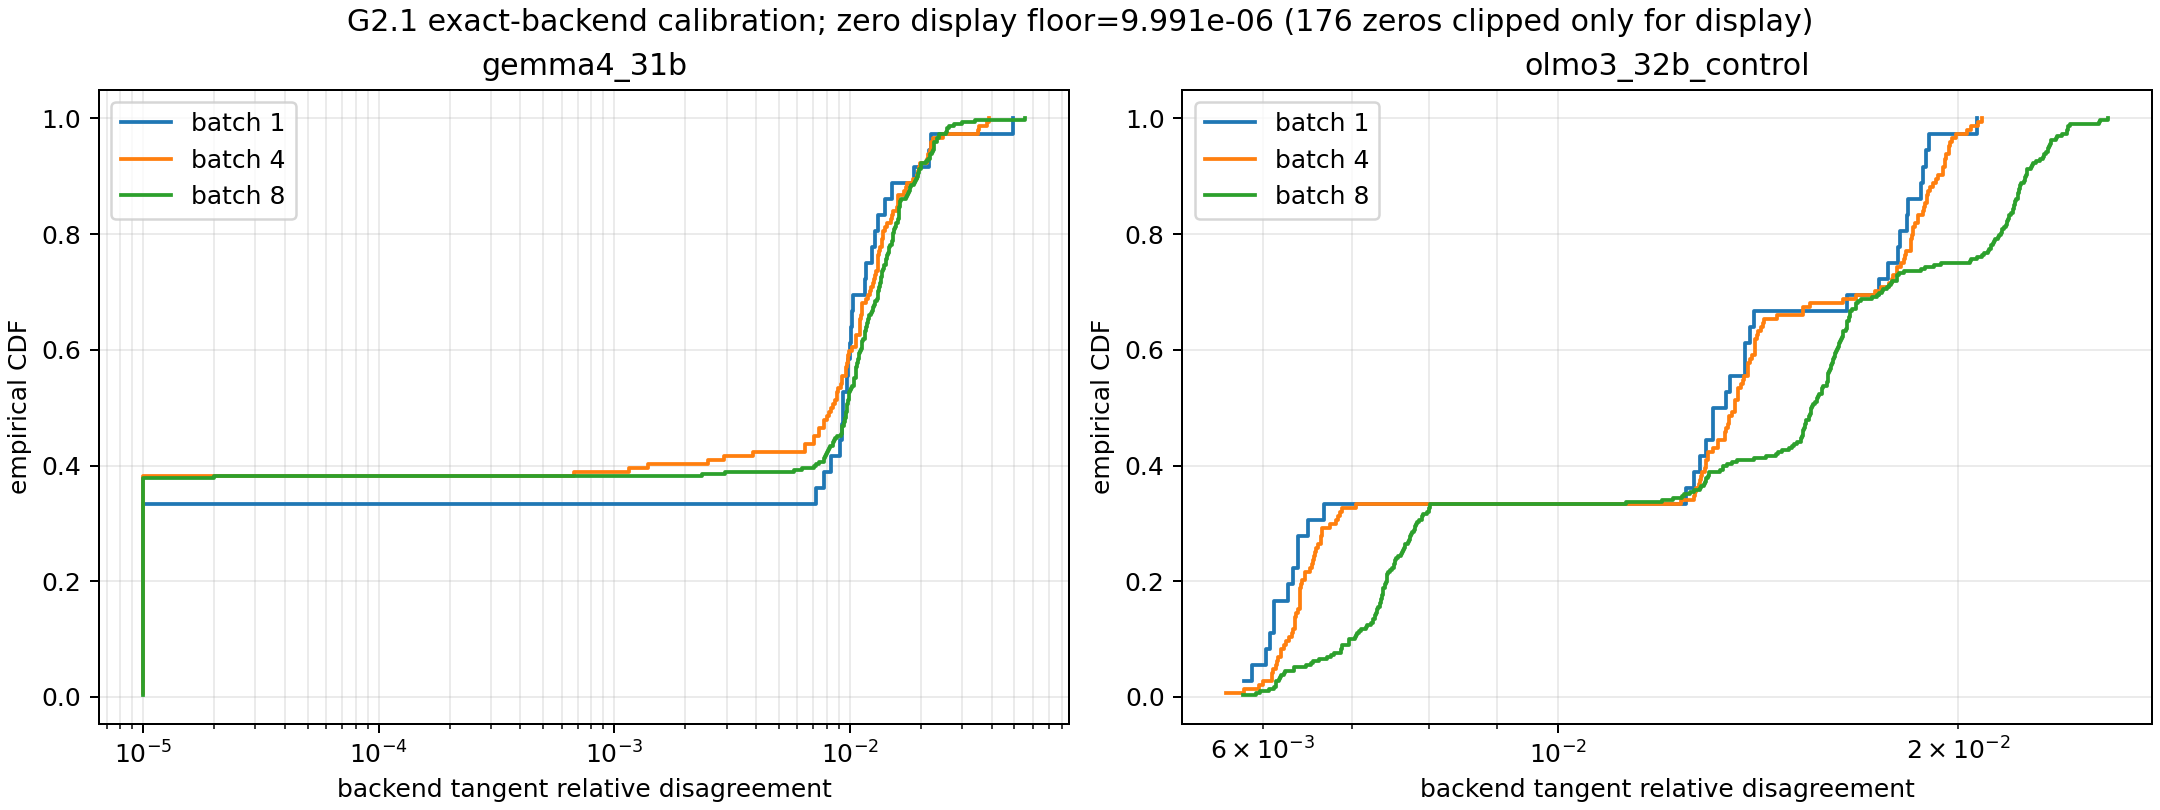
\includegraphics[width=0.96\linewidth]{figures/gm2_backend_disagreement_by_model_batch.png}
  \caption{Registered G2.1 exact-backend disagreement by model and batch. The
  log-scale display clips exact zeros only for plotting; no scientific value
  or summary is modified.}
\end{figure}

\section{Study 2: mechanical Stage-1 license}
Only after the threshold file was frozen and G2.1 registered did G2.2 open the
hash-pinned Study-1 artifacts. The historical all-slot relative error is
0.0024581113830208778, below the calibrated ceiling, while the selected
scientific slot remains bit-identical. The router therefore selects the
prewritten no-recompute relicense branch; no G2.2 model compute is performed.

The unchanged L22/L30/L37/L44/L52
\texttt{local\_tangent\_mismatch} classifications are licensed as a closed
exact-JVP finite-scale methods result on the tested prompts, directions,
final-residual target map, and doses. In compact paper language: at the tested
prompts, layers, directions, and intervention-relevant finite scales, the
prompt-specific first-order tangent of the chosen source-to-target residual
map predicts Gemma's finite response substantially less accurately than the
same estimator predicts the OLMo control; the mismatch changes character with
depth.

\section{Boundary and continuity}
Study 2 supersedes the Study-1 handoff classification, not its evidence. The
original stop was correct under its own precommitted gate. The new license was
derived under a separate target firewall and cannot be read as retroactive
threshold tuning. It establishes neither nondifferentiability nor the absence
of a Jacobian, information, or a workspace, and it does not identify curvature,
routing, normalization, attention, gated-MLP, or context heterogeneity as the
cause. Both studies remain development/methods tier and open no confirmatory
cell or intervention.
\end{document}
